\documentclass[draft=false
              ,paper=a4
              ,twoside=false
              ,fontsize=11pt
              ,headsepline
              ,BCOR10mm
              ,DIV11
              ]{scrbook}
\usepackage[ngerman,english]{babel}
%% see http://www.tex.ac.uk/cgi-bin/texfaq2html?label=uselmfonts
\usepackage[T1]{fontenc}
\usepackage[utf8]{inputenc}
%\usepackage[latin1]{inputenc}
\usepackage{libertine}
\usepackage{pifont}
\usepackage{microtype}
\usepackage{textcomp}
\usepackage[german,refpage]{nomencl}
\usepackage{setspace}
\usepackage{makeidx}
\usepackage{listings}
\usepackage{natbib}
\usepackage[ngerman,colorlinks=true]{hyperref}
\usepackage{soul}
\usepackage{hawstyle}
\usepackage{lipsum} %% for sample text
% Better table
\usepackage{tabularx}

% Better itemize
\usepackage{enumitem}

% For minipages with figures %%
\usepackage{caption}          %
\usepackage{subcaption}       %
%%%%%%%%%%%%%%%%%%%%%%%%%%%%%%%

%% define some colors
\colorlet{BackgroundColor}{gray!20}
\colorlet{KeywordColor}{blue}
\colorlet{CommentColor}{black!60}
%% for tables
\colorlet{HeadColor}{gray!60}
\colorlet{Color1}{blue!10}
\colorlet{Color2}{white}

%% configure colors
\HAWifprinter{
  \colorlet{BackgroundColor}{gray!20}
  \colorlet{KeywordColor}{black}
  \colorlet{CommentColor}{gray}
  % for tables
  \colorlet{HeadColor}{gray!60}
  \colorlet{Color1}{gray!40}
  \colorlet{Color2}{white}
}{}
\lstset{%
  numbers=left,
  numberstyle=\tiny,
  stepnumber=1,
  numbersep=5pt,
  basicstyle=\ttfamily\small,
  keywordstyle=\color{KeywordColor}\bfseries,
  identifierstyle=\color{black},
  commentstyle=\color{CommentColor},
  backgroundcolor=\color{BackgroundColor},
  captionpos=b,
  fontadjust=true
}
\lstset{escapeinside={(*@}{@*)}, % used to enter latex code inside listings
        morekeywords={uint32_t, int32_t}
}
\ifpdfoutput{
  \hypersetup{bookmarksopen=false,bookmarksnumbered,linktocpage}
}{}

%% more fancy C++
\DeclareRobustCommand{\cxx}{C\raisebox{0.25ex}{{\scriptsize +\kern-0.25ex +}}}

%% TODOS markieren
\newcommand{\TODO}[1]{\colorbox{yellow}{\textcolor{red}{[TODO: #1]}}}

\clubpenalty=10000
\widowpenalty=10000
\displaywidowpenalty=10000

% unknown hyphenations
\hyphenation{
}

%% recalculate text area
\typearea[current]{last}

\makeindex
\makenomenclature

\begin{document}
\selectlanguage{ngerman}

%%%%%
%% customize (see readme.pdf for supported values)
\HAWThesisProperties{Author={Benjamin Burchard}
                    ,Title={Evaluation und Analyse von Visualisierungen und Visualisierungswerkzeugen für die Netzwerkkommunikation im Fahrzeug}
                    ,EnglishTitle={Evaluation and analysis of visualisation tools and technics for network communication in vehicles}
                    ,ThesisType={Master Arbeit}
                    ,ExaminationType={Master Ausarbeitung}
                    ,DegreeProgramme={Master of Science Informatik}
                    ,ThesisExperts={Prof. Dr. Franz Korf}
                    ,ReleaseDate={19. März 2017}
                  }

%% title
\frontmatter

%% output title page
\maketitle

\onehalfspacing

%% add abstract pages
%% note: this is one command on multiple lines
\HAWAbstractPage
%% German abstract
{Schlüsselwort 1, Schlüsselwort 2}%
{Dieses Dokument \ldots}
%% English abstract
{keyword 1, keyword 2}%
{This document \ldots}

\newpage
\singlespacing

\tableofcontents
\newpage
%% enable if these lists should be shown on their own page
%%\listoftables
\listoffigures
%\lstlistoflistings

%% main
\mainmatter
\onehalfspacing

\chapter{Einleitung} % (fold)
\label{cha:einleitung}
Die Visualisierung von Daten zielt darauf ab, Informationen durch eine grafische Interpretation verwertbar zu machen.
\iffalse
Es soll eine Evaluation von Informationssystemen und Visualisierungen stattfinden und deren Vergleich mit dem eigenen Prototypen (sowie dessen Erweiterung zu einem Informationssystem(?)). 

\TODO{Auch noch Teile aus Einleitung AW2? Soll RT Ethernet und dass Fahrzeug mit einbezogen werden? Denke Ja.}

\TODO{REVIEW + UMSCHREIBEN}
Visualisierung bietet viele Mittel um Daten einen Sinn zu verleihen. Das Abbilden der Datenattribute auf visuelle Eigenschaften wie Position, Form, Farbe und Größe wird eingesetzt um Nutzern die Wahrnehmung und Interpretation von Mustern innerhalb der Daten zu erleichtern \cite{shneiderman_designing_2005}. Damit visuelle Analyse Tools effektiv genutzt werden können, müssen diese eine fließende und flexible Nutzung von Visualisierungen ermöglichen. Um das zu ermöglichen wird in \cite{heer_interactive_2012} eine \textit{Taxonomy of interactive dynamics for visual analysis} eingeführt. Diese ist in drei Kategorien eingeteilt welche die kritischen Aufgaben der visuellen Analyse beschreiben. Die Kategorien sind \textit{Data and View Specification}, \textit{View Manipulation} sowie \textit{Process and Provenance}. Die erste Kategorie beschäftigt sich mit den spezifischen Daten und Views welche für die jeweiligen Bedürfnisse der Analysten von Interesse sind. Es muss eine Steuerung der Applikation ermöglicht werden, so dass die Daten selektiv visualisiert werden können, irrelevante Daten herausgefiltert werden und ebenso müssen die Informationen sortiert werden können um mögliche Muster erkennbar zu machen. Nach der Erstellung einer Visualisierung muss es den Analysten ermöglicht werden die gestellten Views nach Bedürfnis zu manipulieren, dies beschreibt die zweite Kategorie der Taxonomy. Die Manipulation der Visualisierung ist nötig um Muster aufzeigen zu können, Hypothesen zu untersuchen und zur Navigation in den Daten bspw. via Drilldown. Analyse Tools muss es möglich sein multiple verbundene Visualisierungen zu organisieren und zu koordinieren um mehr Einsicht in Multidimensionale Daten zu bieten als es isolierte Views vermögen. Dies wird schon im häufig zitierten Mantra von Ben Shneiderman vorgegeben: "\textit{Overview first, zoom and filter, then details-on-demand}" \cite{shneiderman_the_eyes_1996}. Die abschließende Kategorie \textit{Process and Provenance} beschreibt den iterativen Prozess der Datenexploration sowie den der Dateninterpretation. Wenn Analysten Ihre bisher getätigten Aktionen innerhalb eines Programms nachverfolgen können kann die Arbeit überprüft und verbessert werden. Es sollte möglich sein die Ergebnisse zu dokumentieren als auch diese mit anderen zu teilen um eine Diskussion darüber zu ermöglichen. Ferner können Analysewerkzeuge auch Anfänger durch Ihre Funktionen führen um die Benutzung und den Einstieg zu erleichtern.
Die vorgegebene Taxonomie bietet einen guten Einstiegs- und Orientierungspunkt in der Welt der Visualisierung und kann ebenso als Checkliste bei der Entwicklung eines neuen Analysetools verwendet werden. Sie zeigt viele Möglichkeiten auf um den Daten Herr werden zu können. \TODO{REVIEW + UMSCHREIBEN}
% chapter einleitung (end)
\fi

Im Kapitel \ref{cha:umfeldanalyse} wird grob das Wissenschaftliche \TODO{und wirtschaftliche?} Umfeld umrissen. In drei Unterabschnitten werden hier die Grundlagen und angrenzenden Wissensbereiche dieser Arbeit beleuchtet. Inwiefern die Wahl der richtigen Evaluationsmethode die Qualität der Ergebnisse und der möglichen Schlussfolgerungen beeinflusst. Aktuelle und bewährte Konzepte der eingesetzten Ethernet Netzwerke, sowie deren Methoden zur Visualisierung von Kommunikationsdaten in Bereichen der Flugzeugtechnik, der ... sowie der... werden erörtert, als auch die Anforderungen und die Analyse dieser betrachtet. \TODO{Das vielleicht mit in Section Evaluation -> Section: Evaluation und Anforderungsanalyse} \TODO{oder: Evaluation und die Bedeutung für Schlussfolgerungen und Anforderungen}
Kapitel \ref{cha:evaluationsbasis} vergleicht verschiedene Evaluationstechniken und erläutert den Aufbau und die Herangehensweise dieser. Im Verlauf des Kapitels wird Aufgrund von verschiedenen Analysen anderer Wissenschaftlicher Ausarbeitungen eine Evaluationsmethode gewählt. Diese wird zur Evaluation für die im Kapitel \nameref{cha:literaturauswertung} vorgestellten akademischen Abhandlungen verwendet. Das oben genannte Kapitel \ref{cha:literaturauswertung} beinhaltet die erwähnte Literaturauswertung, mit Hilfe der erarbeiteten Evaluationstechnik werden diese Arbeiten aufgearbeitet. Das anschließende Kapitel \ref{cha:anforderungsanalyse} greift die in Kapitel \ref{cha:literaturauswertung} gewonnenen Erkenntnisse auf und es werden darauf basierend Anforderungen für die Darstellung von Netzwerkdaten im Fahrzeug-Ethernet erstellt. Aufgeteilt wird dieses Kapitel in drei Schritte. Zunächst werden allgemeingültige Anforderungen vorgestellt, gefolgt von Anforderungen speziell für den Visualisierungsbereich. Im Anschluss werden konkrete Anforderungen an Visualisierungen von Netzwerkdaten im Fahrzeug gestellt. Kapitel \ref{cha:auswahlkriterien} \TODO{möglich in Kapitel 5 rein..}
Das Kapitel \ref{cha:anwendungskonzepte_und_bereiche} beschreibt welche Anwendungsmöglichkeiten sich aus der Anforderungsanalyse ergeben und wie, als auch wo, diese Kombiniert und eingesetzt werden können. Kapitel \ref{cha:zusammenfassung_und_fazit} schließt diese Arbeit mit einer Zusammenfassung und einem Fazit ab.

\chapter{Umfeldanalyse} % (fold)
\label{cha:umfeldanalyse}
Im der \nameref{cha:einleitung} wurde erläutert warum Visualisierungen für die Darstellung der Netzwerkkommunikationsdaten im Fahrzeug wichtig sind. Dieses Kapitel skizziert die Position dieser Arbeit im Bezug auf das wissenschaftliche Umfeld. Der Kernbereich beschäftigt sich mit Visualisierungen aus dem Automotive Bereich. Im speziellen mit Darstellungen für die Kommunikation im modernen Automotive Realtime Ethernet. Neben diesem Hauptbereich gibt es mehrere weitere angrenzende Themen die für die Arbeit von Bedeutung sind. In der folgenden Übersicht \ref{fig:theme_overview} sind diese Bereiche dargestellt. Das Umfeld ist im Wesentlichen in drei Teile gegliedert, Evaluation, Werkzeuge und Visualisierungen sowie Anforderungen und die Analyse dieser. 

\begin{figure}[htbp]
  \centering
  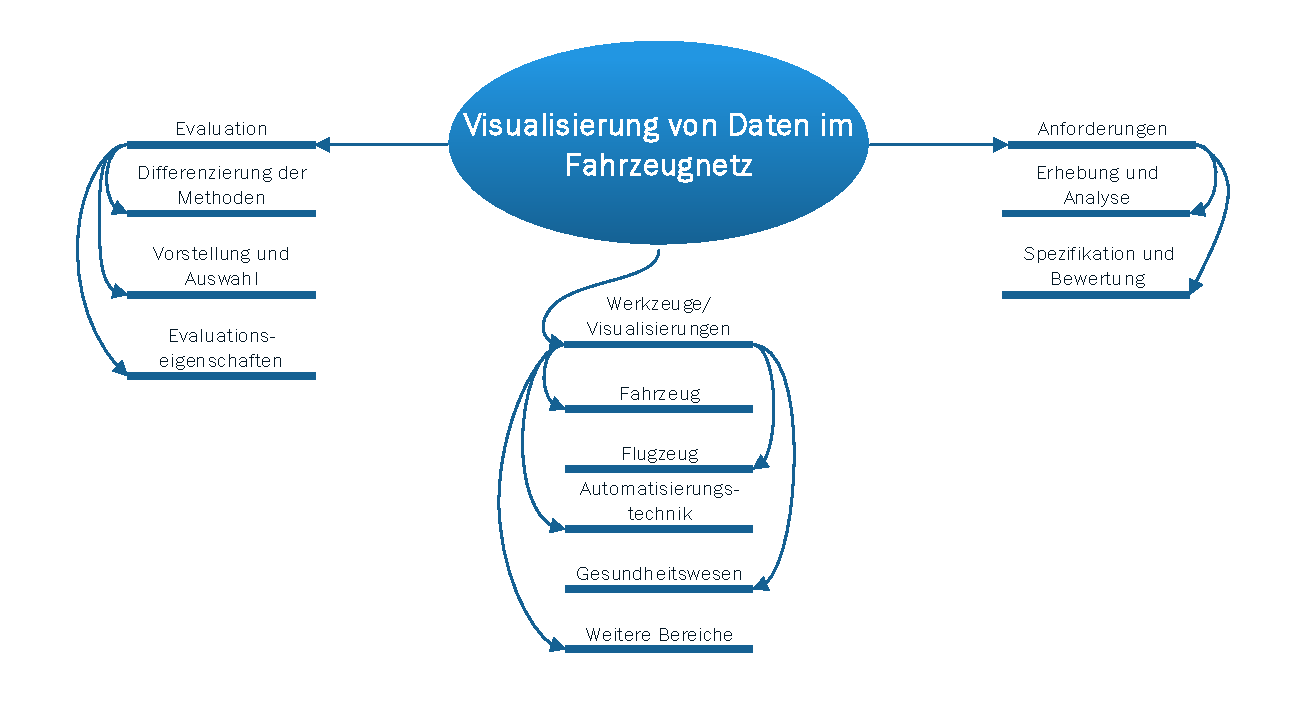
\includegraphics[width=\textwidth]{img/theme_overview.pdf}
  \caption{An diese Arbeit angrenzende wissenschaftliche und wirtschaftliche Bereiche}
  \label{fig:theme_overview}
\end{figure}

Im Abschnitt \ref{sec:evaluation} wird erläutert warum die Evaluation der Visualisierungen und Werkzeuge notwendig ist und die Vorarbeit für das Kapitel \nameref{cha:evaluationsbasis} geleistet, welches die geeignetste Technik für die Visualisierung von Netzwerkdaten im Fahrzeugnetz herausarbeitet. Abschnitt \ref{sec:visualisierungen_und_werkzeuge} beschreibt die Notwendigkeit der Betrachtung von Visualisierungen und Werkzeugen nicht nur aus dem Automotive Bereich sondern auch aus angrenzenden Bereichen. Der Abschnitt befasst sich weiterhin damit welches diese Bereiche sind und warum diese in Frage kommen. Der abschließende Teil dieses Kapitels, \nameref{sec:anforderungen_und_analyse}, geht auf die Anforderungen an Visualisierungen ein. Es wird \dots 

\section{Evaluation} % (fold)
\label{sec:evaluation}

Im Bereich der Evaluation beschäftigt sich die Arbeit mit der Frage welche Techniken zur Evaluation sinnvoll in diesem Themenkomplex einsetzbar sind. Bereits das folgende Kapitel \ref{cha:evaluationsbasis} beschäftigt sich mit der Basis für eine Evaluation der Werkzeuge und Visualisierungen, welche hauptsächlich aus dem Bereich der Fahrzeugkommunikation stammen. Es wird herausgearbeitet welche Evaluationsmöglichkeiten es gibt und welche, aufgrund Ihrer Ergebnisse und Anwendungsgebiete, am geeignetsten erscheinen. Die Wahl der Art der Evaluation ist entscheidend, weil diese darüber entscheidet in welcher Art und Weise die Ergebnisse genutzt werden können. Diese Entscheidung wird von mehreren Faktoren beeinträchtigt. Den Zielen welche mit der Methode erreicht werden sollen, die Umstände und Grenzen die der Evaluationsaufgabe auferlegt sind und der Charakteristik der Objekte welche evaluiert werden sollen. Diese unterschiedlichen Faktoren interagieren miteinander was die Wahl der geeignetsten Evaluationsmethode schwierig gestaltet \cite{kitchenham_evaluating_1996-2}. Kitchenham hat bereits Mitte der neunziger Jahre neun verschiedene Evaluierungsverfahren ausgemacht. 

4. Qualitative screening: A feature-based evaluation done by a  single individual who not only determines the features to be assessed and their rating scale but also does the assessment. For  initial screening, the evalua- tions are usually based  on literature describing the soft- ware method/tools rather than actual use of the meth- ods/too KITCHENHAM1

au empirical studies, lam et al
\begin{itemize}
  \item scope of eval: prototype , e.g., to see if a visualization has achieved
its design goals, to see how a prototype compares with
the current state-of-the-art systems or techniques.
\end{itemize}
\TODO{...}
\TODO{Beispiele}
% section evaluation (end)

\section{Visualisierungen und Werkzeuge} % (fold)
\label{sec:visualisierungen_und_werkzeuge}

Visualisierungen und Werkzeuge wie zum Beispiel Informationssysteme werden in vielen Bereichen der Wissenschaft und Wirtschaft eingesetzt. Dieser Abschnitt möchte einen Überblick über angrenzende Wissensbereiche schaffen und dortige Methoden und Werkzeuge analysieren. 
Naheliegender angrenzende Bereiche sind jene aus dem Verkehrswesen. In der Flugzeugtechnik wird bereits mit Ethernet im Flugzeugnetz experimentiert und es ist auch schon im Einsatz, beispielsweise im A380 oder der Boeing 787. Auch hier wurde der erhöhte Kommunikationsbedarf erkannt und mit einem auf die Luftfahrt spezialisiertem und von Airbus entwickelten Datennetz reagiert. Das sogenannte Avionics Full-Duplex Switched Ethernet (AFDX) wird hauptsächlich für sicherheitskritische Anwendungen verwendet \cite{steiner_recent_2014}. 


\TODO{...}

% section visualisierungen_und_werkzeuge (end)

\section{Anforderungen und Analyse} % (fold)
\label{sec:anforderungen_und_analyse}

Visueller Analyse Bereich muss auch noch eingegrenzt werden

% section anforderungen_und_analyse (end)

\section{Zielsetzung der Arbeit} % (fold)
\label{sec:zielsetzung_der_arbeit}
Diese Arbeit hat zum Ziel Evaluationstechniken in Hinblick auf deren Einsatzfähigkeit im Feld der Visualisierung von Fahrzeugkommunikationsdaten und deren Werkzeuge zu Analysieren. Unter Zuhilfenahme der erarbeiteten Evaluationstechniken wird spezifische Literatur ausgewertet. Damit ist gemeint das hier Literatur speziell aus dem Bereich der Netzwerkvisualisierung ausgewertet wird, mit Hauptaugenmerk auf die Darstellung von Kommunikationsdaten im Fahrzeug. Aus der Analyse der Literatur ergeben sich Anforderungen an Visualisierungen für den Automotive Bereich, welche Aufgearbeitet werden und somit eine Grundlage für die Entwicklung neuer Visualisierungssystemen und Werkzeuge bilden. 
Somit ergeben sich mehrere konkrete Teilziele dieser Arbeit. Es werden geeignete Evaluationstechniken für die Analyse von Werkzeugen und Visualisierungen im Bereich der Visualisierung von Fahrzeugkommunikation erarbeitet. Es werden konkrete Anforderungen für zukünftige und aktuelle Darstellungsformen und die zugehörige Software zusammengestellt.
% section zielsetzung_der_arbeit (end)
% chapter umfeldanalyse (end)

\chapter{Evaluationsbasis} % (fold)
\label{cha:evaluationsbasis}
In den letzten 20 Jahren beschäftigten sich über 80\% der Evaluationen bezüglich der Visualisierung und ihrer Werkzeuge mit den sich ergebenden Bildern und mit der Performance der verwendeten Algorithmen. Allerdings lassen mehr und mehr Evaluationen Teilnehmer in ihren Studien partizipieren. Von den Teilnehmern wird dann die Leistungen sowie das subjektive Feedback Evaluiert oder es wird ihre (verbesserte) Performance mit der Visualisierung und in der Analyse, als auch bei der Fähigkeit zur Schlussfolgerung berücksichtigt \cite{isenberg_systematic_2013}. 

Lam et al. haben in ihrer Ausarbeitung \cite{lam_empirical_2012} 850 Paper hinsichtlich möglicher Evaluierungsszenarien untersucht. Sie haben sieben verschiedene Szenarien ermittelt, welche sich in zwei grundlegende Kategorien aufteilen. Zum einen gibt es Szenarien, welche mit dem Verständnis der eigentlichen Visualisierungen beschäftigen, zum anderen solche die zum Nachvollziehen der Datenanalyse dienen. Besonders das Szenario aus der Datenanalyse \textbf{evaluating visual data analysis and reasoning (VDAR)} sticht für die angestrebte Arbeit heraus. Evaluationen in diesem Bereich fokussieren sich hauptsächlich darauf ob und wie ein Visualisierungswerkzeug visuelle Analysen und Schlussfolgerungen über Daten zulässt. Mögliche Ergebnisse sind hierbei sowohl Metriken (bspw. Anzahl der Analyseerkenntnisse), als auch subjektives Feedback (bspw. Umfrage über Datenanalysequalität). Meist werden in diesem Bereich Feldstudien genutzt, häufig in der Form von Fallstudien.


\iffalse

Wie Eval andere? -> Kriterien / Nutzen?

Aus verschiedenen Evaluationsmöglichkeiten ergeben sich verschiedene Anforderungen

Evaluierungsszenarien und Evaluierungspraktiken

\fi

\section{Evaluationsansätze} % (fold)
\label{sec:evaluationsansätze}
dies sind die Ansätze die es so gibt

% section evaluationsansätze (end)
\section{Entscheidung für Evaluationsansatz} % (fold)
\label{sec:entscheidung_für_evaluationsansatz}
dieser oder die Kombi aus diesen ist für Automotive am besten weil! Und dieser wird für die Literaturanalyse bzw. Analyse von bestehenden Visualisierungen und Werkzeugen verwendet.

% section entscheidung_für_evaluationsansatz (end)
% chapter evaluationsbasis (end)

\chapter{Literaturauswertung} % (fold)
\label{cha:literaturauswertung}

Dieses Kapitel beleuchtet die für diese Arbeit relevante Literatur. Das Kapitel ist in zwei Bereiche gegliedert, zum einem werden theoretische Abhandlungen betrachtet welche sich mit Anforderungen an vornehmlich Netzwerk bezogenen Visualisierungen beschäftigen. Zum Anderen...

\section{Verwandte Arbeiten} % (fold)
\label{sec:verwandte_arbeiten}
\iffalse
In einer Studie von Sedlmair et al. \cite{sedlmair2009} wurden ausgewählte Darstellungsarten auf ihren Zuspruch für ein Expertenpublikum getestet. Besonders hervorzuheben ist hier der neu kreierte Autobahnview. Der Autobahn View zeigt den Datenstrom der Bussysteme (die Autobahn). Jeder Bus transportiert Nachrichten verschiedener ECUs, dargestellt als horizontale Linie (eine Fahrbahn der Autobahn). Wobei die Daten als Nachrichten, in Form von kleinen Rechtecken (die Fahrzeuge), dargestellt werden. Adaptiert auf ein Ethernet-Backbone Netz, wären die Virtuellen Links die Autobahn, ein einzelner Link eine Fahrbahn und genauso wie ursprünglich wäre eine Nachricht ein Fahrzeug. Damit lassen sich beispielsweise der zyklische Datenverkehr beobachten, das Verständnis für Fahrzeugnetze erweitern, Ursache-Wirkung Relationen untersuchen sowie die gesamte Fahrzeugkommunikation beobachten. Aufgrund der starken Nachfrage und der großen Breite an möglichen Anwendungsgebieten für die Autobahn Darstellungsform, ist es ein Ziel diese in der nächsten Version des Prototypen, möglicherweise in der  anschließenden Masterarbeit, zu verwirklichen. \TODO{Rewrite, has to be included}
% section verwandte_arbeiten (end)
\fi
\section{Visualisierungen und Werkzeuge} % (fold)
\label{sec:anwendungen_und_werkzeuge}
Es wurde bereits eine große Zahl an verschiedensten Analyse-Werkzeugen entwickelt. Dieser Abschnitt geht auf die Funktion, die Nutzbarkeit und das Anwendungsgebiet der für diese Arbeit relevanten Programme ein. Die Programme kommen aus den verschiedensten Bereichen, der Automatisierungstechnik, der Flug- und Fahrzeugindustrie so wie weiteren kleineren Bereichen. Es handelt sich dabei sowohl um proprietäre, als auch um wissenschaftlich erarbeitete Anwendungen. 
\iffalse\TODO{RLY? Recap if still true}\fi

Cardiogram \cite{sedlmair_cardiogram:_2011} ist eine Software, die speziell zur Darstellung von Daten im Automotiven Bereich entwickelt wurde. Es visualisiert Fehler in Prototypen-Tests über Logfiles, welche während reellen Testfahrten entstehen. In dieser Arbeit von Sedlmaier et al. gibt es bereits erste Ansätze zum Umgang mit großen Datenmengen im Gigabyte Bereich, wie automatisierte Datenfilterung und -abstraktion über State Machines sowie automatisierte Fehlererkennung.\TODO{detaillierter}


In der neuesten Arbeit von Lajmi et al. \cite{lajmi_using_2013} wurde Ethernet bereits zur Netzwerkanalyse innerhalb eines Fahrzeugs genutzt. Hier wurde ein Netzwerktool ähnlich zu WireShark, namentlich CableFish, entwickelt. Die Software erkennt bereits neuartige Protokolle der Automobilindustrie, wie z.B. SOME-IP \cite{someip_scalable_2014}, und ist gedacht als Unterstützung für Diagnosetools. Allerdings werden hier zwar mit Hilfe von Ethernet Daten empfangen, es wurden allerdings die Daten der fahrzeugspezifischen Protokolle, wie LIN, CAN und FlexRay in Ethernetpakete verpackt. Des Weiteren wurde dieses Programm bisher nur in einer simulierten Umgebung getestet, hat aber eine verbesserte Echtzeitfähigkeit. Da für wurde ein weiterer Buffer vor der Datenspeicherung eingebaut und so die Anzahl der Systemaufrufe reduziert. \TODO{DETAILS}
% section anwendungen_und_werkzeuge (end)
% chapter literaturauswertung (end)

\chapter{Anforderungsanalyse} % (fold)
\label{cha:anforderungsanalyse}
Wie hilft diese Vis Technik/Werkzeug bei welchem Fehler oder Beobachtung auch immer?

Motivation für diese Anforderung?

80:20! welche 20\% Anf. sind für 80\% der Infos verantwortlich??\newline
->>>> SCALABILITY;STORYTELLING?;EFFECTIV EVAL?

A systematic review -> 2. Absatz in Conclusion \cite{isenberg_systematic_2013} \newline
empirical studies in \cite{lam_empirical_2012}

\section{Allgemeine Anforderungen} % (fold)
\label{sec:allgemeine_anforderungen}
Dieser Abschnitt soll die unterschiedlichen Anforderungen welche an Visualisierungswerkzeuge, ebenso wie an Visualisierungstechniken gestellt werden, herausarbeiten. Im folgenden werden dann die essentiellen Anforderungen hervorgehoben um in einem letzten Schritt diese auf ihre Anwendbarkeit im Automotivebereich geprüft.


\subsection{Anforderungen an Visualisierungen} % (fold)
\label{sub:anforderungen_an_visualisierungen}

Anforderungen an Visualisierungen:

\begin{itemize}
  \item Verständlichkeit und schneller Zugriff auf Daten
  \item Zeitersparnis bei der Analyse
  \item Kollaboratives Arbeiten
  \item Datenabstraktion, Überblick über Daten
\end{itemize}
% subsection anforderungen_an_visualisierungen (end)

\subsection{Anforderungen an Werkzeuge} % (fold)
\label{sub:anforderungen_an_werkzeuge}

Spez. Anforderungen an Werkzeuge:

\begin{itemize}
  \item Große Datenmengen verarbeiten/Datenexploration 
  \item Neue Erkenntnisse schaffen
  \item Visuelle Analysen mit Schlussfolgerungen über Daten
\end{itemize}

\TODO{ANMERKEN: SEHR SEHR ALLGEMEIN, SINN? }
% subsection anforderungen_an_werkzeuge (end)


% section allgemeine_anforderungen (end)
\section{Automotive spezifische Anforderungen} % (fold)
\label{sec:automotive_spezifische_anforderungen}
Visualisierungen Automotive spezifischer:

\begin{itemize}
  \item Verbesserte temporale Struktur und Orientierung
    \begin{itemize}
    \item schnellere Übersicht
    \item bessere Navigationsmöglichkeiten als in Liste
    \item grobe sowie feine Zeitinformationen nötig
  \end{itemize}
  \item Zugriff auf Rohdaten muss gegeben sein
  \begin{itemize}
    \item Signale, Nachrichten und deren Werte müssen abrufbar sein
    \item Abstraktion kann helfen, aber nicht um Werte aus Rohdaten anzuzeigen
  \end{itemize}
\end{itemize}

Werkzeuge mögliche Evaluierungsrichtungen:

\begin{itemize}
  \item Verständnis der Umgebung und Arbeitspraktiken (In welchem Kontext wird es verwendet? Welche Vis?)
  \item Evaluation der visuellen Datenanalyse und Schlussfolgerungen (Entscheidungsfindung, Hypothesengenerierung, Wie wird das unterstützt?)
  \item 
\end{itemize}
% section automotive_spezifische_anforderungen (end)
% chapter anforderungsanalyse (end)

\chapter{Auswahlkriterien} % (fold)
\label{cha:auswahlkriterien}
\TODO{Das eher als section in Anforderungsanalyse?}
Hier steht das Ergebnis der Anforderungsanalyse. Welche Anforderungen möchte ich anführen für eine Entwicklung von Visualisierungen und Visualisierungswerkzeugen im Fahrzeugnetzbereich.
% chapter auswahlkriterien (end)

\chapter{Anwendungskonzepte und -bereiche} % (fold)
\label{cha:anwendungskonzepte_und_bereiche}

Würde man es nach dem und dem Ansatz machen wäre das ergebnis so und so

kombiniert man den und diesen Ansatz dann wäre das so

daraus ergibt sich (hoffentlich) ein völlig neuer Ansatz
% chapter anwendungskonzepte_und_bereiche (end)

\chapter{Zusammenfassung und Fazit} % (fold)
\label{cha:zusammenfassung_und_fazit}

% chapter zusammenfassung_und_fazit (end)

\backmatter

\typeout{===== Section: literature}
%% read the documentation for customizing the style
\bibliographystyle{abbrv}
\bibliography{ausarbeitung_haw}

\typeout{===== Section: nomenclature}
%% uncomment if a TOC entry is needed
%%\addcontentsline{toc}{chapter}{Glossar}
\renewcommand{\nomname}{Glossar}
\clearpage
\markboth{\nomname}{\nomname} %% see nomencl doc, page 9, section 4.1
\printnomenclature

%% index
\typeout{===== Section: index}
\printindex

\HAWasurency

\end{document}
